\chapter{\mFourL: A measurement designed for re-interpretation}
\label{chap:fourlepton}

\chapterquote{Very inspiring quote}
{Very inspiring quote author}

%% LHC and ATLAS introduction
\section{The \LHC and the \ATLAS experiment}
\label{sec:LHCandATLAS}

The massive fruit of labour, decades in the making from the hundreds of institutions which make up CERN, lies hidden 100 meters below the surface of the Switzerland-France border. Sandwiched between Geneva and the Jura Mountains is a 27 km ring of superconducting magnets and radio-frequency (RF) cavities, which bend and accelerate particles to 0.999999991$c$. Mathematically, this is approximately 3 metres per second slower than the speed of light. This remarkable achievement is none other than the Large Hadron Collider (LHC). The LHC lives up to its name; it is the largest machine built by humankind, and unsurprisingly the most powerful high-energy particle collider in the world. The four main interaction points around the ring where particles collide mark the four main experiments: ATLAS, CMS, LHCb, and ALICE. The former two are general purpose detectors with a similar goal: to precisely study the Standard Model and to search for evidence of new physics. The latter two have specialized purposes. LHCb is dedicated to probing physics involving b-hadrons in pp collisions, and ALICE’s aim is to shed light on the physics of the quark-gluon plasma by investigating heavy-ion collisions. 

Prior to the injection into the LHC, the protons first pass through a series of smaller machines which boost them to higher and higher energy. The first in the chain is LINAC2, a linear accelerator that spouts protons (the source of which is hydrogen atoms with electrons stripped away) at \unit{50}{\MeV}. Next the protons are piped into the Proton Synchrotron Booster, the Proton Synchrotron, and finally into the Super Proton Synchrotron \todo{Give more details about each of these steps}. Through this chain the protons get boosted to \unit{1.4}{\GeV} by the PSB, then further to \unit{25}{\GeV} by the PS, to a final \unit{450}{\GeV} by the SPS before entering the LHC. Inside the pipes of the LHC, the protons take a short 20 minutes to reach \unit{6.5}{\TeV}. 

\begin{figure}
  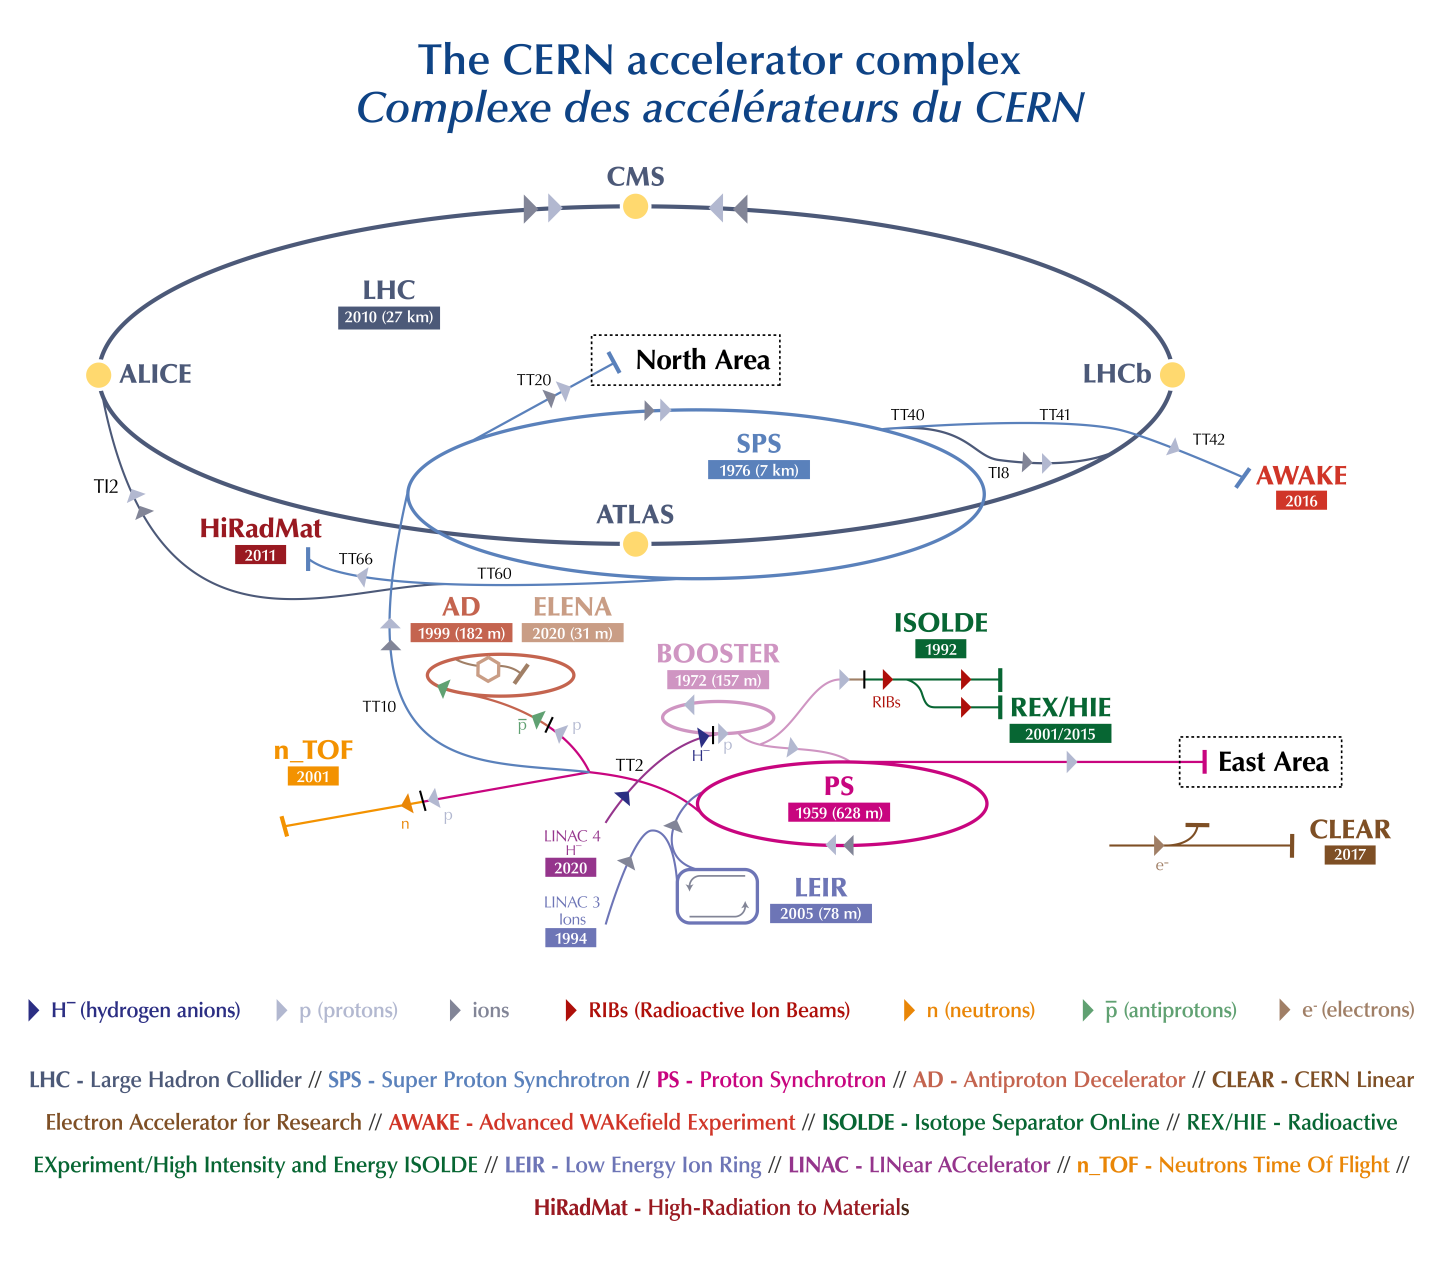
\includegraphics[width=\mediumfigwidth]{Figures/LHC/CernAcceleratorComplex.png}
  \caption[The \CERN accelerator complex]%
  {The CERN accelerator complex, where the LHC is the largest ring. The four main collision points corresponding to the main experiments are dotted in yellow.}
  \label{fig:CERNComplex}
\end{figure}

The impressive feat of accelerating particles is made possible through the use of radio-frequency cavities. The idea was first crafted by the young Rolf Wideröe \cite{Vretenar:2012} \todo{https://cds.cern.ch/record/1415638/} for his PhD thesis and later caught the eye of the brilliant E. Lawrence, recipient of the Nobel Prize in Physics in 1939 for the invention of the cyclotron. RF cavities are round chambers along the beam. A voltage generator generate a voltage which oscillates at 400 megahertz (MHz), inducing an electric field inside the RF cavity. As particles pass through they experience the force of the field and are accelerated along the beam pipe. In total the LHC uses 8 RF cavities per beam (so 16 in total), with each cavity capable of delivering a 2 megavolts (MV). Protons travelling through the cavity increase their energy to 14 times the injection amount, from 450 GeV to 6.5 TeV. Once protons get up to speed, a proton that has perfect timing will stay put, while protons that arrive slightly earlier/later will be accelerated/decelerate. The result is a beam of protons sorted into smaller segments of proton bunches. The LHC produces two such proton beams, one circulating clockwise and the other counterclockwise. 

An important key concept in particle physics is luminosity. It is a factor that relates the cross-section to the number of event per second, written as follows:
$$\luminosity=\dfrac{1}{\sigma}\cdot\dfrac{dN}{dt}$$
where \luminosity is the luminosity, $N$ is the number of events, and $\sigma$ is the production cross section. The dimension of luminosity is events per unit time and unit area \unit{}{\cm\rpsquared}\unit{}{\second\rp}.

There are two properties used to describe a particle beam: its \todo{write more about this} emittance $\epsilon$, and its $\beta$ function. The emittance can be thought of as the area occupied by the particle beam in the position momentum plane. A lower emittance means the distance between particles and the difference in momentum between the particles are small. The cross sectional sizes of the beam $\sigma_i$ ($i=x,y$) are written as 
$$\sigma_i=\sqrt{\dfrac{\beta_i\cdot\epsilon_i}{\pi}}$$ The beams are assumed to be Gaussian distributed, meaning that in collisions, the centres of the beams contribute most while the edges have minimal impact. Following this the luminosity is
$$\luminosity=\dfrac{N_1N_2f_{rev}N_b}{2\pi\Sigma_x\Sigma_y}$$
where $N_1$ and $N_2$ are the number of particles for each bunch, $N_b$ is the number of bunches, $f$ is the revolution frequency, and $\Sigma_x,\Sigma_y$ represent the \unsure{Erm what is a convolution..?} convolution of the beam sizes. They can be expressed as
$$\Sigma_x=\sqrt{\sigma_{x1}^2+\sigma_{x2}^2}, \quad \Sigma_y=\sqrt{\sigma_{y1}^2+\sigma_{y2}^2}.$$
Assuming that the beam sizes are identical and round, $\sigma_{x1}=\sigma_{x2}=\sigma_{y1}=\sigma_{y2}$, and the luminosity becomes
$$\luminosity=\dfrac{N_1N_2f_{rev}N_b}{4\pi\sigma^2}=\dfrac{N_1N_2f_{rev}N_b\gamma}{4\pi\epsilon_N\beta^*}$$

When proton beams cross at the LHC, there are many collisions which occur other than the hard-scatter of interest. While increasing the number of particles per bunch increases the likelihood of a rare interaction, it also increases the pile-up of multiple interactions. Pile-up, denoted as $\mu$, is one of the biggest obstacles for LHC experiments; the more there is, the more difficult it becomes to disentangle the events of interest from the sea of low energy collision. The contribution to pile-up events can be separated into two main categories: 
\begin{itemize}
  \item In-time pile-up refers to simultaneous proton-proton collisions occurring in the same bunch crossing as the hard scatter of interest;
  \item Out-of-time pile-up is the overlay of events from neighbouring bunches which contaminate signal events, attributed to detector electronics latency.
\end{itemize}
There are also less-substantial contributions from the cavern background, beam halo events, and beam gas events. The cavern background is the cloud of gas that floods the LHC cavern during operation. Beam halo events are from when the proton beam interacts with the collimating instrumentation, and the beam gas events describe interactions between the beam and the residual gas in the beam pipe. 

By the end of Run II at the \LHC, the pile-up \todo{Write about pile-up}.
%% m4l motivation
\section{Motivation for the \mFourL measurement}
\label{sec:fourlepmotivation}

The idea behind this analysis is to make a measurement as inclusive and as model-independent as possible. The fiducial region definition follows closely the acceptance of the detector. Furthermore, by loosening the mass cuts, there is higher event acceptance especially in the low mass regions. Preliminary studies were conducted to investigate the impact of loosening and simplifying the dilepton lower mass cut to \unit{5}{GeV} and removing the upper mass cut, for example, as opposed to the varying higher cuts in the previous round of the analysis. Unsurprisingly, these result in a higher event yield in both the low and high mass tails of the \mFourL distribution. 

%% Theoretical predictions 
\section{Theoretical predictions}
\label{sec:theory}

Theoretical predictions from Monte Carlo simulations

%% Signal definition and event selection
\section{Signal definition and event selection}
\label{sec:signaldef}

The final state is defined solely in terms of final state particles as opposed to targeting a specific process. Beyond the requirement of two same flavour opposite sign lepton pairs, the measurement is inclusive to additional particles such as additional leptons, jets, and invisible particles. Previous irreducible backgrounds (\VVV, \ttZ) are now considered as part of the signal since they produce four or more prompt leptons.

\section{Background estimation}
\label{sec:background}

\section{Systematic uncertainties}
\label{sec:sysuncert}

%% Unfolding and respective studies
\section{Unfolding}
\label{sec:unfolding}

To unfold a measurement means to correct it for detector-effects, since what the detector sees is not what truly occurs in nature. Rather, data at the detector-level include additional side effects that one must consider, such as resolution effects, detector acceptance, etc. On the simulation side, detector simulations are the most computationally expensive. For re-interpretation purposes, having to run through the entire detector simulation chain for every model of interest is highly inefficient. Furthermore as detector technology advances and changes, as does the simulation software. In order to re-interpret detector level data published in a certain year, one would have to use the simulation software corresponding to what was in use back then. 

It is desirable to unfold Standard Model measurements so that it can be used and compared to theoretical predictions in years to come. By presenting measurements at the particle level, no further simulation is require beyond the raw output of the event generator, which is a big advantage. 

\subsection{Unfolding methodology}
\label{subsec:unfmethod}

\subsection{Binning optimization}
\label{subsec:binningopt}

The binnings of the measured distributions were optimized based on two factors: the number of events and the purity of each bin. Here the purity refers to the diagonal of the migration matrix normalised along truth, thus representing the fraction of truth events that end up in the same reconstructed event bin. There were several iterations of the binning that were run with varying criteria, summarised in table \ref{tab:BinningVersions}.

The first iteration of the binnings were run with the Default criteria. Here, depending on the number of events in the bin, the purity requirement varies. Bins with lower statistics have a high purity requirement to reduce bin-to-bin migrations. The minimum number of events required for each bin is 10. Between 10 and 15 events, the purity was required to be at least 80\%. Between 15 and 20 events the purity must be 70\% or higher. Finally for bins with more than 20 events the purity cut was 60\%. 

The binning algorithm is as follows. For the full \mFourL differential mass distribution from \unit{20}{\Gev} - \unit{2000}{\GeV}, the distribution was first split into very fine steps of \unit{1}{\GeV} bins from \unit{20}{\Gev}-\unit{450}{\GeV}. From \unit{450}{\Gev}-\unit{2000}{\GeV} wider steps of \unit{5}{\GeV} bins were used. Due to the fine nature of the bin widths, this initial binning failed to meet any of the binning criteria. Next, the binning algorithm starts from the low mass end and starts to merge adjacent bins together if the criteria were not met. For example, if bin number 1 [20,21] has > 10 events, the algorithm merges bin number 1 with the next bin. The new bin number 1 is now [20,22]. Once again, if this bin has > 10 events, it will merge again and become [20,23], and so on and so forth until 10 events has been reached. Of course the purity must also pass the required percentage for the number of events in the bin, otherwise further bin merging occurs.  

Next we have the \mFourL distributions in double differential slices of \ptFourL, \yFourL, and flavour channel. For these distributions, the fine binning is defined as the the binning of the full \mFourL differential mass distribution, i.e. the output of the algorithm described in the previous paragraph. Bins were once again checked for number events and purity, and merged as needed. This was implemented so that all \mFourL in each of the  \ptFourL, \yFourL, and flavour slices would have bin edges that match with the inclusive distribution. 

For the distributions measured double differentially in the four \mFourL regions corresponding to \Z, \Higgs, On-shell \ZZ, and Off-shell \ZZ, the same procedure was followed for binning optimisation. Each distribution had a fine binning defined, and the bins were merged from left to right of the x-axis until the criteria were met. 

\begin{table}[bp]
  \begin{tabular}{lllll}
                & Default              & Stringent              & High statistics             \\
    \midrule
                                & 10 (purity > 0.8)   & 14 &   \\
     Minimum number of events & 15 (purity > 0.7) & 20 & 100    \\
                                &20 (purity > 0.6) & 25 &    \\
  \end{tabular}
  \caption{Three different versions of binning with varying criteria.}
  \label{tab:BinningVersions}
\end{table}

\subsection{Pre-unfolding weights}
\label{subsec:preuf}

\subsection{Injection tests}
\label{subsec:injection}



\section{Results}
\label{sec:results}

Results plots